
%%%%%%%%%%%%%%%%%%%%%%% file typeinst.tex %%%%%%%%%%%%%%%%%%%%%%%%%
%
% This is the LaTeX source for the instructions to authors using
% the LaTeX document class 'llncs.cls' for contributions to
% the Lecture Notes in Computer Sciences series.
% http://www.springer.com/lncs       Springer Heidelberg 2006/05/04
%
% It may be used as a template for your own input - copy it
% to a new file with a new name and use it as the basis
% for your article.
%
% NB: the document class 'llncs' has its own and detailed documentation, see
% ftp://ftp.springer.de/data/pubftp/pub/tex/latex/llncs/latex2e/llncsdoc.pdf
%
%%%%%%%%%%%%%%%%%%%%%%%%%%%%%%%%%%%%%%%%%%%%%%%%%%%%%%%%%%%%%%%%%%%

\documentclass[runningheads,a4paper]{llncs}
    
%\usepackage[garamond]{mathdesign}
\usepackage{varwidth}
\usepackage{linegoal}
\usepackage{POE}
\usepackage{amssymb}
\usepackage{amsmath}
\usepackage{comment}
%\newtheorem{comment}{comment}[section]
%\setcounter{tocdepth}{3}
\usepackage{graphicx}
\usepackage[textsize=tiny,textwidth=\marginparwidth]{todonotes}
%\newcommand{\hookdownarrow}{\mathrel{\rotatebox[origin=b]{-270}{$\hookleftarrow$}}}

\usepackage{url}
\newcommand{\keywords}[1]{\par\addvspace\baselineskip
\noindent\keywordname\enspace\ignorespaces#1}

%\usepackage [autostyle=true, english=british]{csquotes}
%\MakeOuterQuote{	}

\usepackage{NewItMathFont}
\renewcommand*{\mprintsingle}[2]{\mathit{#1}}%
\renewcommand*{\mprintmulti}[2]{\mathit{#1}}%

\usepackage[inline]{enumitem}
\usepackage{wrapfig}

%\input{problems}

\begin{document}

\mainmatter

\title{POE-$\Delta$: Towards an engineering framework for solving change problems}
\titlerunning{POE-$\Delta$}

\author{Georgi \textsc{Markov} \and Jon G. \textsc{Hall} \and Lucia \textsc{Rapanotti}}
\authorrunning{Markov, Hall, Rapanotti}


\institute{Department of Computing and Communications\\ 
The Open University, UK\\
\url{{georgi.markov, jon.hall, lucia.rapanotti}@open.ac.uk}
}

\toctitle{POE-$\Delta$: Towards an engineering framework for dealing with change problems}
\tocauthor{Markov, Hall, Rapanotti}
\maketitle


\begin{abstract}
Many organisational problems are addressed through change to existing Information Systems rather than radical new design. In the face of up to 70\% IT project failure, devising effective ways to tackle this type of change remains an open challenge.
The paper discusses the motivation, theoretical foundation, characteristics and evaluation of a novel framework - referred to as POE-$\Delta$, which is rooted in design and engineering and is aimed at providing systematic support for representing, structuring and exploring change problems.
We generalise an existing theory of greenfield design as problem solving for application to change problems, using a design science research methodology. From a theoretical perspective POE-$\Delta$ is a subset of its parent framework, allowing the seamless integration of greenfield and brownfield design to tackle change problems. Its initial case study evaluation shows that POE-$\Delta$ allows the systematic analysis of change problems, leading to clearer understanding and more informed decision making.

%\textbf{\\Context:} Many organisational problems are addressed through change to Information Systems rather than their radical design. In the face of up to 70\% IT project failure, devising effective ways to tackle complex change problems remains an open challenge. 
%
%\textbf{Objective:} The paper discusses the motivation, theoretical foundation, characteristics and early evaluation of a novel framework, rooted in design and engineering, which we refer to as POE-$\Delta$ and which is aimed at providing systematic support for representing, structuring and iteratively exploring a change problem. 
%
%\textbf{Method:} We generalise an existing theory of greenfield design as problem solving for application to change problems, using a design research methodology. As part of the evaluation phase, a case study approach is taken in the context of a real-world organisation The case study concerns the adoption of the Open Services for Lifecycle Collaboration (OSLC) interoperability standard in one of the organisation's own tools.
%
%\textbf{Results:} The paper demonstrates how from a theoretical perspective POE-$\Delta$ is a subset of its parent framework, allowing the seamless integration of greenfield and brownfield design to tackle change problems. From a practical viewpoint, the case study evaluation shows how POE-$\Delta$ allows the practitioner to systematically analyse a change problem of realistic complexity, leading to clearer understanding and more informed decision making by stakeholders as to where an intervention was necessary for solution. 
%
%\textbf{Conclusion:} The results are encouraging, in that, while acknowledging the limitations of a single case study,  they demonstrate that the framework allows the systematic analysis of a need to change through  an understanding of: how the change impacts the domains that will need to be modified by the solution; the domains that will indirectly influence or be influenced by it or as a result of its introduction to the organisation; and those domains that will remain untouched by the change. However, clear difficulties were also highlighted, including the question of scalability of the graphical notation and automatability of the analysis process which will be the focus of future research.
\keywords{organisational change, information systems, change problems, problem solving, design theory}
\end{abstract}

\section{Introduction}
Continuous change is part of the make-up of the  modern organisation, and crucial to its survival and success in an ever-increasing competitive and volitile business environment. Information systems are often at the heart of organisational change, either as drivers or enablers, in their essential role within complex organisational socio-technical systems. This has led to the introduction of a multitude of approaches and theories on how to approach organisational change successfully. Yet, a large proportion of change initiatives end in failure \cite{burnes2011success}: while the reasons are many and complex, some have been attributed to a lack of systematic guidance and direction, particularly in key re-design steps which are part of the change process \cite{doi:10.1108/14637159910249117}, \cite{Reijers2005283}, \cite{Gerrits:1994:BMB:646303.686971}. To remedy this deficiency, some have advocated the need for a structured, detailed design theory from which detailed methods can be derived to guide the change process \cite{verkerk2004trust}, \cite{Kleiner:2000vm}, \cite{By:2005fm}. The work presented in this paper makes a contribution towards addressing this challenge.

Our overall research aim is the definition of a framework for addressing change problems systematically, by providing the means to represent, structure and  explore those problems. The framework is rooted in design and engineering, and extends an existing design theoretic framework for problem solving called Problem Oriented Engineering (POE in short, \cite{Hall2012ISSE}), hence its name {\it POE-$\Delta$}. The paper discusses the motivation, theoretical foundation, characteristics and early evaluation of POE-$\Delta$.

From a methodological perspective we take a design science approach \cite{Hevner:2010ua}, starting from an initial theoretical proposition based on POE, followed by empirical evaluation in the form of a case study in the context of a real-world organisation. 

The remainder of this paper is organised as follows. Section \ref{sect:Background}, as mentioned, discusses some background literature. Section~\ref{sect:POEDelta} introduces POE-$\Delta$ and details of its initial evaluation. A discussion is given in  \ref{sect:Discussion}, while \ref{sect:Conclusion} concludes the paper. 

\section{Background} \label{sect:Background}

\subsection{Organisational change}
In the field of Management Science organisational change is defined as ``the process of continually renewing an organisation's direction, structure, and capabilities to serve the ever-changing needs of external and internal customers'' \cite{Moran:2000ex}. It has been the subject of study since the early 1950s, resulting in a multitude of approaches and theories on how it can be successfully tackled (see, e.g., reviews in \cite{vandeVen:1995uw} and \cite{pettigrew2001studying}). While there are significant differences between these approaches, a common criticism is that they only provide very high level change process descriptions to guide the organisation through change initiatives, and by and large are rather imprecise and unmethodical, and that this is true of even influential approaches adopted in practice, such as Total Quality Management (TQM) and Business Process Reengineering (BPR) \cite{Cao:2004dh}. Specific criticisms include: a lack of ``a systematic approach that can lead a process redesigner through a series of steps for the achievement of process redesign'' \cite{doi:10.1108/14637159910249117}; a lack of ``actual technical direction to (re)design a business process'' \cite{Reijers2005283}; a limitation to ``descriptions of the `situation before' and the `situation after', giving very little information on the redesign process itself'' \cite{Gerrits:1994:BMB:646303.686971}.

Many have advocated the need for {\it design thinking} \cite{rowe1991design} in organisational change, and indeed this has become increasingly topical, with many articles discussing its role as an enabling concept which can be embedded within a development approach to organisational change (see, e.g., \cite{3460223} or \cite{deserti2014design}). However, still lacking is a design theory and systematic methods to make the re-design process more structured, easier to operationalise and less dependent on the creativity and intuition of single individuals, a clear objective advocated by some \cite{verkerk2004trust,Kleiner:2000vm}. A number of other contributions, for instance \cite{grover1993information}, \cite{limam2007best}, \cite{reijers2005best}, \cite{berio2001enterprise}, describe best practices, heuristics, and models aimed at supporting the re-design process which can be used to bring more structure into the re-design process. With the notable exception of Aals and Hee's work on using colored Petri-Net to model and analyse business processes \cite{van1996business}, all other works we have reviewed come short of discussing how these techniques can be applied and integrated as part of a comprehensive methodology which provides guidance on the redesign process for practitioners and formalism to analyse change and its effect on the organisation. This is where our research comes in.

\subsection{Contributions}
The management science conceptualisation of organisational change  as a ``difference in form, quality, or state over time in an organizational entity'' \cite{Van-de-Ven:2017aa} is suggestive of a benchmark approach to change: ``measure the same entity at two or more points in time on a set of dimensions and then calculate the differences.'' The dimensions can be sophisticated: number of employees, IT systems, geographical locations, etc., but are change agnostic: they are affected by change, but not aligned with it.

In our approach, an organisation is characterised as a tangle of solved problems, with its future determined by the solving of problems it faces. This is a change-aligned view of the organisation – change consists of tangle understanding, problem understanding, problem solving and, finally, solution insertion into the tangle.
 
\begin{itemize}
	\item Contribution to knowledge
	A key theoretical contribution of this research is approaching organisational change from a design theoretic perspective by applying design problem solving techniques to it. We define a new problem solving methodology for change problems, \POE{}-$\Delta$, to aid users in systematically analysing and solving change problems by helping them to better represent, structure, and explore them to pinpoint where intervention is necessary and what the ramification of that intervention could be. For this, \POE{}-$\Delta$ builds on \POE{}, an existing problem solving methodology for greenfield problem, and reframes it in the context of change (or brownfield) problems. This includes adaptations to POE's problem representation and analysis means, reinterpretation of its process pattern, extensions to its problem transformation patterns, as well as the definition of novel approaches to capture and explore co-design dependencies during the process of problem transformation, and while still remaining compatible to the parent framework, \POE{}. 
	\item Contribution to practice
	Additionally, the research aims to contribute to practice by gathering empirical evidence within real-world organisations as to the practicality and effectiveness of the new methodology. For this, we are currently in the process of preparing a comparison and an evaluation of \POE{}-$\Delta$ against other popular organisational change methodologies. The evaluation will be performed on a complex, real-live change problem in the context of a large, multinational IT organisation and will involve the participation of employees from different countries and at different levels of the organisation.
\end{itemize}

\subsection{Design Problem Solving}\label{design}

Design problems were defined by \cite{jonassen2000toward} as real-world problems which are ill-stuctured and complex. Ill-structuredness implies that the starting point is often vague goals and intentions, with unclear success criteria, hence many degrees of freedom in the problem statement and no unique path to solution \cite{simon1977structure}%,goel1989motivating}
. Complexity refers to the number of issues and variables involved and their relationships, but also to their stability over time and uncertainty which is beyond the problem solver's grasp or control \cite{funke1991solving}%,fischer2011process}
: as such complexity also relates to how difficult a problem is to solve for a human problem solver.

With its origin in engineering and system sciences, the notion of design problem has been extended to any design artefact, whether a physical product or a system or just a course of action \cite{smith1993conceptual}. In this sense, some have argued that many organisational problems \cite{martin2009design},\cite{leavy2010design} can be seen as design problems. 

Design problem solving \cite{smith1993conceptual}  has been explored widely in the context of creating a new artefact, whether a physical product or a system or a course of action \cite{smith1993conceptual}, so-called {\it greenfield} design. Design problem solving for {\it brownfield} design, that is design aimed at changing a current solution in order to meet some new need in context, remains under-explored. With our research we contribute a systematisation of design problem solving in the case of change problems. 

%In doing so, we rely on seminal work by Smith and Browne \cite{smith1993conceptual} that, on the basis of an extended critical review of the literature of the time, distilled a conceptual foundation of design problem solving with respect to salient features of design problems and the design activity to address them. Briefly, design problem solving needs to cope with their complexity and ill-structuredness, and must: 
%\begin{itemize}
%\item 	allow the explication of the relationship between unsatisfied needs which motivate, inform, and instigate the design activity, and provide evaluation criteria for the designed artefact, and constraints which determine what is feasible by establishing relationships between properties of the designed artefact and its context; 
%\item be able to capture constraints which arise both from the context and as part of the design activity; 
%\item allow for alternatives, generated via experiential knowledge (personal and/or collective) and creative imagination, alongside reasoned analysis;
%\item allow for representation of many forms and many languages, which may change throughout the design activity, with precision increasing as problem solving progresses;
%\item allow for a notion of satisficing \cite{simon1996sciences}, intended as establishing some threshold of acceptability of a solution by stakeholders, which does not necessarily imply logical satisfaction or optimality.
%\end{itemize}
  
\subsection{POE}\label{sect:POE}

\POE{}, defined by the second and third authors, is an engineering framework with an accumulated body of work spanning over a decade, including application and evaluation through a number of real-world engineering case studies. Its underlying design theory concerns the characterisation of individual problems and how problems relate and transform to other problems as part of problem solving processes. A thorough presentation of POE is beyond the scope of this paper, but can be found in \cite{hall2016a-design}. Here, we briefly recall some basic definitions, extended by POE-$\Delta$ to change problems in Section~\ref{sect:POEDelta}.

A POE problem is ``a stakeholder's recognised need in context.'' For stakeholder $G$, with recognised need $N_G$ in real world context $E_G$, we defined their problem to be the pair:
%
\[(E_G,N_G)\]
%

$E_G$ and $N_G$ are to be understood only as place holders, as $G$'s initial conceptualisation of their problem may have neither solution nor sense. Irrespective of sense or solution existence, $G$'s wish becomes a challenge to designer $D$ to make sense of $G$'s problem by finding an agreed environment $E$ and need $N$, leading to $D$'s problem
%
\[E(S)\meets_{G}N\]
%
which reads ``Find $S$ which, when installed in $E$, meets $N$ to the satisfaction of $G$.''

$D$'s challenge consists of all the solving problems activities that lead to the solution of $G$'s problem. Someway through problem solving we encounter $D$'s variously detailed $E$, $N$ and $S$ and form a judgement as to whether a problem has been solved. We do this by creating a solution for it through a sequence of judgement-preserving transformations, i.e., transformations that the relevant stakeholders would agree preserved solvability, that move a problem to known solved problems. Thus, a problem is solved if and only if it can be transformed to known solved problems. As part of the transformation sequence, a solution to the problem is created.

Treatment of the physical world in POE is based on the work of Jackson and others \cite{896248}, \cite{Jackson2001}, \cite{hall2003reference}, which relies on the notion of real-world phenomena and their relationships. For the purpose of this discussion, a phenomenon can be simply characterised as ``an element of what we can observe in the world.'' Hence a problem environment $E$ is a set of \textit{domains}, each a set of related \textit{phenomena} that are usefully treated as a unit for the purpose of problem solving (c.f., \cite[Page 270]{Jackson2001}). As a structure, an environment $E$ is a collection of  domains $[D_{1},...,D_{n}]$. Domains interact through their sharing of phenomena; behaviourally, a domain maps a collection of phenomena to a timeline of their occurrences and interactions \cite{hall2003reference}.

The POE problem solving process proceeds through a set of identifiable development steps, which are instances of recurrent problem transformation types, e.g. sensemaking \cite{weick1995sensemaking}. These are defined as ``software problem transformation schema,'' each describing a general way in which a problem may be related to other problem(s). While  POE transformation schema are beyond the scope of this paper, in Section~\ref{sect:POEDelta} we will see examples in the context of POE-$\Delta$.

\section{POE-$\Delta$}
\label{sect:POEDelta}
\POE{}-$\Delta$ shares and extends a number of \POE{}'s characteristics, including elements of its semantics; its graphical notations; and its underlying process pattern \cite{Hall2009JAdvSysMeas}. However, while \POE{} deals with `greenfield' development, \POE{}-$\Delta$ deal with change, or  `brownfield,' problems which are solved not solely by the design of a new artefact, but by a change of, and addition to, existing artefacts within a target context (a system, product, process, etc).

\POE{}-$\Delta$'s aim is to support users in systematically analysing and solving change problems by helping them to better represent, structure, and explore them to pinpoint where intervention is necessary and what the ramification of that intervention could be. To achieve this, \POE{}-$\Delta$, offers an entire problem solving methodology in the sense of Smith and Browne \cite{smith1993conceptual}, including means for problem representation, decomposition and exploration of alternative solutions and supported by a process pattern to guide the user through the problem capturing, transformation and validation steps.

In the following we briefly introduce formal elements of \POE{}-$\Delta$ and report on its initial evaluation trough an organisational case study.

\subsection{Background}
\label{theory}

The inspiration behind \POE{} is the definition of Rogers \cite{rogers1983nature}, which is defines \textit{engineering} as:
%
\begin{quotation}
 the practice of organizing the design and construction of any artifice which transforms the physical world around us to meet some recognized need 
\end{quotation}
%
Clearly, Rogers' had in mind greenfield engineering; indeed, \POE{} focusses on the production of the \textit{artifice}. In contrast, \POE{}-$\Delta$ focuses on the \textit{transformation} of the \textit{environment before} $E$ into an \textit{environment after} $F$ which will meet the need.

\POE{}-$\Delta$ imports \POE{}'s notions of need and environment, defined in terms of the domains $\{D_i\}$ located therein, and phenomena. Two domains that share phenomena can thus interact. 
%Thus, associated with each domain $D$ are three phenomena alphabets:
%%
%\begin{itemize}
%	\item the phenomena \textit{controlled} by $D$ but that are shared by other domains. Controlled phenomena are written superscripted, $D^controlled$. 
%	\item the phenomena \textit{observed} by $D$ that are made visible by other domains. Observed phenomena are written subscripted, $D_observed$.
%	\item all other \textit{unshared} phenomena, written parenthesised, $D(unshared)$.
%\end{itemize}

%When controlled and observed phenomena are brought within `hearing distance' of each other they link together.

%A change problem need $N$ states how the after environment $F$ will be assessed as the solution. A need relates phenomena; there are two alphabets associated with it:
%\begin{itemize}
%	\item $refs$: those phenomena that are referenced (but not constrained) by a need description, written subscripted.
%	\item $cons$: those phenomena that are constrained by a need description, i.e., those phenomena that the change solution may affect as a solution to the problem.
%\end{itemize}

Phenomena are, clearly, critical to understanding how domains interact. However, they may be elided if the nature of that interaction is otherwise stipulated. Like \POE{}, we prescribe no single description language for a problem's elements; indeed, different elements can be described in different languages. In this paper, we indicate domain connectivity in a number of ways, include the graphical notation that illustrates Section~\ref{sect:ChangeProblemSolving}.

\subsection{A Theory of Change problems}
\label{sect:ChangeProblemSolving}

We begin from the same place as \POE{}\footnote{The presentation loosely follows \cite{hall2016a-design}}: we suppose that change problem owner $G$ recognises a need in the real world and wishes that need to be satisfied. From $G$'s perspective, then, a  problem $P$ is a pair, consisting of a real world context $E_G$ and a need $N_G$. We make no assumption that $G$'s view of the real world context is realistic or representable, nor that $G$'s recognised need has a solution. 

Irrespective of sense or solution existence, we will assume that $G$'s wish becomes a challenge to a change engineer $D$ to make sense of $G$'s change problem $(E_G,N_G)$ and to solve it. $D$'s challenge thus consists of (cf. \cite{hall2016a-design}):
%
\begin{enumerate}[label=CPS\arabic*.]
%\begin{enumerate}
	\item creating their own view, $(E, N)$, of the $G$'s change problem $(E_G, N_G)$;
	\item receiving validation from $G$ that $(E, N)$ is properly representative;
	\item identifying a new environment $F$ consisting of i) those the parts of $E$ that can remain unchanged, together with ii) changes to $E$, and iii) any additions necessary to effect the change;
	\item receiving validation from $G$ that $F$ meets the agreed recognised need $N$;
	\item migrating from $E$ to $F$.
\end{enumerate}

Even if expressed linearly as bullet points, the challenge facing $D$ may be iterative and highly non-linear.

\newcommand\CM{Pixel}
\def\ColourMaker#{\textit{ColourMaker} (shortly \textit{CoMa})\gdef\ColourMaker{\textit{CoMa}}}
\newcommand{\code}[1]{\texttt{#1}}
\newcommand{\solved}{\relax}
\newcommand{\replacedBy}{\triangleright}
\newcommand{\Java}{Swift}

Given the above, we consider a change problem to be a four-tuple, written $E\Delta F\meets_G N$ where $E$ and $F$ are both collections of domains and $N$ is a need. Unlike $E$ which is arrived at from an understanding of the real world, $F$ is a designed object, created through iteration of the steps CPS3 and CPS4. As such, and without constraining the languages in which existing and new components are or will be expressed, it is constrained in the forms it can take which are defined by the following grammar:
%
\[\footnotesize\begin{array}{rcll}
	ChangeDomain &:=& Domain \mid Domain[\{Changeable\}](\{NewDomain\})\\
	Changeable &:=& ChangeDomain \mid CP \mid \cancel{Domain} \mid Domain \replacedBy NewDomain\\
	Domain, NewDomain, Need &:=& Name
\end{array}\]
%
\begin{wrapfigure}{r}{0.45\textwidth}
\centering{
	 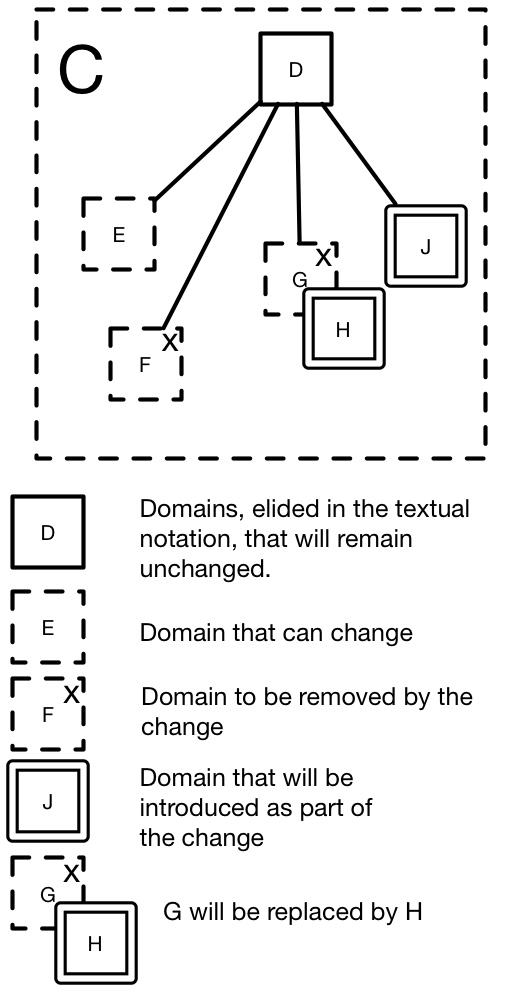
\includegraphics[width=0.39\textwidth]{pics/GraphicalNotation}}
  \caption{The \textit{ChangeDomain} notational conventions}
  \label{fig:notationIllustration}
\end{wrapfigure}
There are a number of representational conventions in the above grammar (illustrated in Figure~\ref{fig:notationIllustration}). Suppose the (hierarchical) domain $C=[D,E,F,G]$. Then:
\begin{enumerate}
	\item ($\{\}$) is written $()$; 
	\item in the first clause of the $Change$ $Domain$ production, domain $C$ is undecorated. This identifies $C$ as a changeable domain, i.e., its embedded domains will be subject to further change analysis;
	\item in the second clause, given $C$, we have an expression such as $C[E, \cancel{F}, G\replacedBy H](J)$, by which we mean:
\begin{enumerate*}[label=(\roman*)]
\item $D$ (elided) remains unchanged; 
\item $E$ is changeable (cf.~the previous clause above);
\item $F$ will be removed by the change; 
\item $G$ will be replaced by $H$ (which, thus, observes and controls the same phenomena as $G$); and 
\item $J$ will be introduced by the change.
\end{enumerate*}
\end{enumerate}


A change problem is said to be \textit{greenfield} whenever each $Changeable$ element is either $\cancel{Domain}$ or $Domain\replacedBy Domain$, i.e., each changeable element is either deleted or replaced. A change problem that isn't greenfield is \textit{brownfield}. Although we do not define the equivalence here, a greenfield change problem is equivalent to a (\textit{tangle} of) \POE{} problem(s) \cite{hall2016a-design}. As we shall see, as well as forging the link with \POE{}, the notion of a greenfield problem is at the core of what it means for a change problem to be solvable.

%\paragraph{Mapping to \POE{}}
\newcommand\zerothCP{E\Delta F\meets_G N}
\newcommand\firstCP{[\Java,\ColourMaker{}]\Delta \ColourMaker{}[CM[\cancel{\alpha}, \cancel{R},\cancel{G},\cancel{B}](\alpha RGB)]()\meets_G RTDNeed}
%

\newcommand{\RTDNeed}{\ensuremath{RTDNeed}}
\newcommand{\GeorgiStepMinusOne}{[\Java,\ColourMaker{}]\Delta F\meets_G \RTDNeed}
%
\begin{example}
A software house's CEO, $G$, is in reflective mood and wishes to reduce the technical debt in \ColourMaker{}, a commercial image manipulation app. Georgi, an experienced software engineer, is tasked with doing so.

Following Step CPS1 (perhaps in collaboration with $G$) Georgi captures the initial change problem in \POE{}-$\Delta$ as:
%
\begin{equation}
	\GeorgiStepMinusOne
\end{equation}
%
in which $[\Java,\ColourMaker]$ is Georgi's understanding of the problem owner's change problem context, i.e., the $\ColourMaker{}$ app and its $\Java$ environment; $\RTDNeed$ is his understanding of their need; and $F$ stands for the new environment that Georgi will create to solve the problem. 

Assuming that the problem owner is willing to validate Georgi's initial change problem (Step CPS2), focus can turn to analysis of the changes needed to solve the problems by creating the new context $F$. If validation was not forthcoming, Georgi would iterate his understanding until either i) he gained validation, or ii) problem solving was ceased.
\end{example}
%%
%\[\zerothCP\]
%%
%and
%
%****\[\footnotesize\firstCP\]
%%
%In the sequel, we show how this change problem is arrived at from $E\Delta F\meets_G N$ through the application of \textit{change problem transformations}.

 
%For instance:
%%
%\[\begin{array}{rcll} 
%	\lefteqn{\firstCP}\\[2ex]
%	&\qquad\mapsto& [\Java,\ColourMaker{}\setminus\{\CM\},\CM\setminus\{\alpha,R,G,B\}](\alpha RGB)\meets_G RTDNeed
%\end{array}\]

\subsection{Change problem transformation}

Following \POE{}, we define change design as the step-wise transformation of change problems. Suppose, then, we have change problems $E\Delta F\meets_G$, $E_i\Delta F_i \meets_{G_i} N_i$, $i = 1 \dots n$, $(n \geq 0)$ and \textit{step rationale} $J$, then we write:

\[\begin{prooftree} 				
	E_1\Delta F_1 \meets_{G_1} N_1 \solved \qquad \dots \qquad E_n \Delta F_n \meets_{G_n} N_n \solved
\using{\steprat{J}}\justifies
	E \Delta F \meets_{G} N \solved
\end{prooftree}\]
%
to mean that $E\Delta F \meets_{G} N$ is solved with \textit{rationale} $(AA_1 \wedge \dots \wedge AA_n) \wedge J$ whenever $E_i \Delta F_i \meets_{G_i} N_i$, $i = 1 \dots n$, $(n \geq 0)$ are solved with rationale $AA_1, \dots, AA_i$ respectively.

Below the line is the conclusion problem; above the line are the premise problems. Steps can be combined to produce entire \textit{change development trees}.

In our change theory, we establish that a change problem is solved when it can be transformed to a collection of solvable greenfield problems via the above transformation. 

As in \POE{}, there are many classes of transformation. One such is {\sc Substitution}:

\paragraph{Substitution} Given a substitution $PS = [A_i/E_i]$ of change problem elements and step rationale $J_{PS}$, we have the substitution step:
%
\def\substitutionstep{
\begin{prooftree}
	P[PS]\solved
\using{\steprat{{\sc Substitution}\textrm{ $J_{PS}$; environment: $E[PS]$, need: $N[PS]$, change: $F[PS]$}}}\justifies
	P\solved
\end{prooftree}}
\[\substitutionstep\]
%
which capture the situation when, if the appropriate stakeholder is satisfied that the substitution is correct, then the original problem will satisfy the stakeholder when the substitution is made. 

A substitution represents, for us, an increase in our knowledge\footnote{Technically, knowledge is validated belief, with validation arriving from the problem owner. It is thus a stakeholder-relative notion.} of the problem element substituted.

Although we do not have space to describe them in this paper, other classes of change problem transformations exist.

\begin{figure}[hbt]
\centering{
  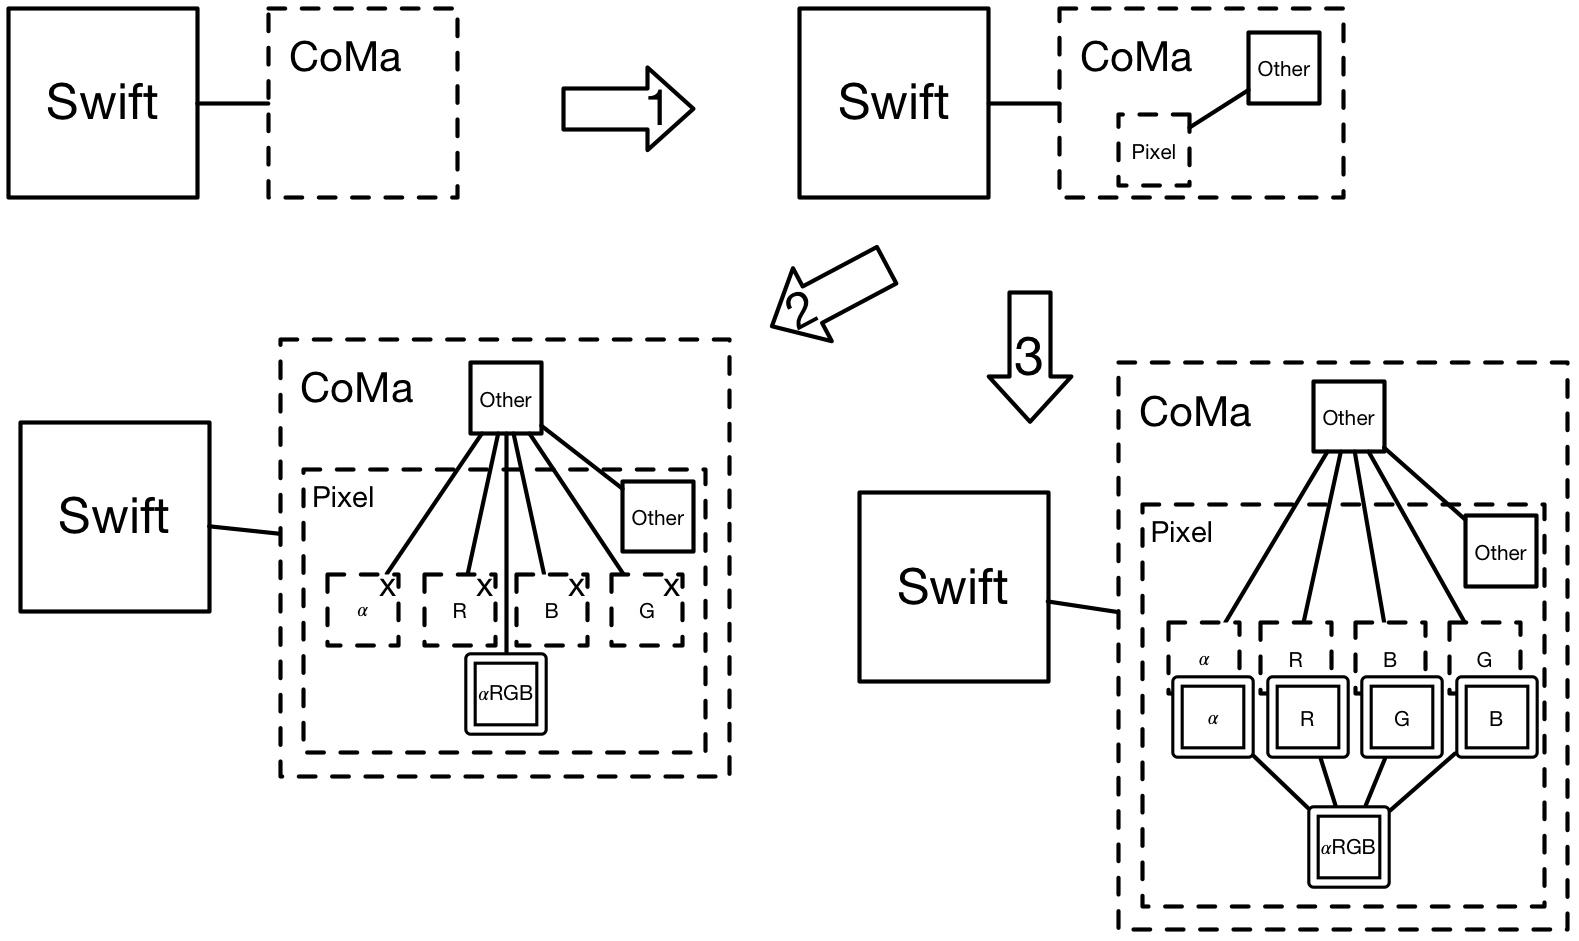
\includegraphics[width=0.7\columnwidth]{pics/SwiftChange}}
  \caption{Illustrating Georgi's change problem; see Example~\ref{ex:two}}
  \label{fig:SwiftChange}
\end{figure}

\newcommand\GeorgiStepZero{[\Java,\ColourMaker{}]\Delta \ColourMaker\meets_G RTDNeed}
\newcommand{\GeorgiStepOne}{[\Java,\ColourMaker{}]\Delta \ColourMaker{}[\CM]()\meets_G RTDNeed}
\newcommand{\GeorgiStepTwo}{[\Java,\ColourMaker{}]\Delta \ColourMaker{}[\CM[\cancel R,\cancel G,\cancel B,\cancel \alpha,](\alpha RGB)]()\meets_G RTDNeed}
\newcommand{\SubsThree}{[\CM/\CM[\cancel R,\cancel G,\cancel B, \cancel\alpha](\alpha RGB)]}
\newcommand{\GeorgiStepThree}{\begin{array}{ll}[\Java,\ColourMaker{}]\Delta \ColourMaker{}[\CM[R\replacedBy R',G\replacedBy G',\\
\qquad\qquad\qquad B\replacedBy B', \alpha\replacedBy\alpha'](\alpha RGB)]()\meets_G RTDNeed\end{array}}

\begin{example}\label{ex:two}
Georgi begins his analysis of the changes needed (Step CPS3). Initially, he identifies that the $\Java$ environment won't need to change in satisfying $\RTDNeed$, but that \ColourMaker{} will. Georgi's first change problem transformation is to apply the substitution $Subs_1=[F/\ColourMaker]$ giving
%
\begin{equation}
\GeorgiStepZero
\label{eqn:backtrack}	
\end{equation}
%
This is the starting point in Figure~\ref{fig:SwiftChange}.

Next, through a detailed code inspection of \ColourMaker, Georgi recognises that the $\CM$ class's getters \code{get\allowbreak RedValue}, \code{get\allowbreak GreenValue}, \code{get\allowbreak BlueValue}, and \code{get\allowbreak AlphaValue} perform the same steps and share significant code, each being distinguished only by their use of different constants in the method bodies. He recognises a recurring software engineering problem for which a best practice remedy is available in the \textit{parameterise method design pattern} \cite{1999:RID:311424} which prescribes the combination of similar methods through a switch parameter. Applying this design pattern will reduce technical debt. Georgi therefore applies the {\sc Substitution} transformation with the substitution $Subs_2=[\ColourMaker/\ColourMaker[\CM]()]$ indicating that the $\CM$ component will be subject of change, whilst leaving the remainder of $\ColourMaker$ unchanged ({\sf Other} in the Figure), giving:
%
\begin{equation}
\GeorgiStepOne
\label{eqn:backtrack2}	
\end{equation}
%
which is Step 1 in Figure~\ref{fig:SwiftChange}.

Initially, Georgi considers reducing technical debt through the substitution\footnote{For brevity, we abbreviate the getters to $R$, $G$, $B$, and $\alpha$, respectively.} $Subs_3=\SubsThree$ which would leave (Step 2):
%
\[\GeorgiStepTwo\]
%
but then realises that, as $\alpha RGB$ has a different signature to each of $R$, $G$, $B$ and $\alpha$, such a change cannot be achieved with changes local to $\CM$, i.e., he would need to consider change to the whole of \ColourMaker{} contradicting the assumption underpinning Equation~\ref{eqn:backtrack} that only $\CM$ would change\footnote{Of course, this assumption might be incorrect, but that could only be established in consultation with $G$ at Step CPS4.}.

Thus, Georgi rejects this choice, backtracking to Equation~\ref{eqn:backtrack} and, instead, reconsiders the substitution $Subs_3$ from which he derives $Subs_4=[\CM/\CM[R\replacedBy R',G\replacedBy G',B\replacedBy B', \alpha\replacedBy\alpha'](\alpha RGB)]$, in which the getters are replaced rather than removed, leaving (Step 3):
%
\[\GeorgiStepThree\]
%


As all changeable domains are either new or replaced, this is now a greenfield problem, for which a solution can be sought for in \POE{}. 

Concatenating the steps Georgi took gives the following change design tree:
%
\[\footnotesize\begin{prooftree}
	\[
		\[
			\GeorgiStepThree
		\using{\steprat{{\sc substitution}, $Subs_4$}}\justifies
			\GeorgiStepOne
		\]
	\using{\steprat{{\sc substitution}, $Subs_2$}}\justifies
		\GeorgiStepZero
	\]
\using{\steprat{{\sc substitution}, $Subs_1$}}\justifies
	\GeorgiStepMinusOne
\end{prooftree}\]

%The equivalent tangle of \POE{} problems is:
%%
%\[\begin{array}{l}}
%[Swift, \ColourMaker\setminus\{\CM\}, \CM\setminus\{R,G,B,\alpha\}](R',G',B',\alpha', \alpha RGB)\]
%	
%\end{array}
\end{example}

\subsection{Real-world Case Study Evaluation}
\label{caseStudy}
%The evaluation of the framework was conducted in form of a case study and aimed at evaluating the applicability and scalability of the \POE{}-$\Delta$ in a real-life context. 
%
%Evaluating the applicability of the framework had the main goal of providing some initial evidence that the framework can be applied to change problems in order to identify elements of the problem's context where a change is necessary, and, in combination with the original \POE{} framework, to guide the design of the change artefact. In doing so, the actual application of the framework and the accompanying process pattern (see \cite{Kaminski:2011wy}) was carried out by the first author while the other relevant problem stakeholders received only sufficient training to read and understand the notation.
%
%The evaluation of the scalability was mainly focused on demonstrating that the framework can successfully be applied to real-world size problems, and that the available notations (both formal and graphical) are able to capture and represent such problems while still remaining readable and useful.

The evaluation case study took place in the context of a multi-national organisation, as contribution to a work package in an EU funded research project\footnote{\url{https://www.eitdigital.eu/innovation-entrepreneurship/cyber-physical-systems/}}. The goal of the work package was to showcase the adoption of the emerging Open Services for Lifecycle Collaboration\footnote{\url{http://openservices.net}} (OSLC) standard in a real-life industrial setting with production-grade tools. The case study organisation led the  work package and provided the tool, a model-based test design editor and generator, for which adoption of the standard was to be realised. Also, as OSLC is intended to enable integration and interoperability between software tools from different tool vendors, the work package required the involvement of, and where appropriate knowledge transfer to, other third-party tool vendors, including at least one SME. 

The whole project took nine months from conception to completion. 5 people were involved in the case study, working in Europe and India. The first author, as principle investigator for the work package, led the POE-$\Delta$ case study work. \POE{}-$\Delta$ was used to identify both technical and organisational changes and to design any new and replacement artefacts needed.

\subsubsection{Objectives}

The main evaluation objectives were to collect early evidence of whether POE-$\Delta$ is:
\begin{itemize}
\item sufficiently expressive for application to a real-world change problem;
\item able to support the systematisation of the problem solving process; and
\item able to cope with real-world complexity.
\end{itemize}

Moreover, we were interested in assessing its performance as a means of communication among project stakeholders, as well as its ability to surface critical design issues to be resolved.

\subsubsection{Procedures}

 At the start of the project the first author introduced POE-$\Delta$ to relevant stakeholders within the organisation, including the project manager, tool architect and several developers. While a formal development was recorded by the first author throughout, only problem descriptions based on the graphical notation (similar, but not identical to, that used in Figure~\ref{fig:SwiftChange}) were shared among project stakeholders. In particular, the notation was used for communication in most technical meetings, but was not used for the upstream communication to project management and external stakeholders.

 The problem solving steps outlined in Section~\ref{sect:POEDelta} were followed, with iteration applied as needed. 
 
 A debriefing with stakeholders, in particular the technical stakeholders who had the most exposure to the framework, was held at the end of the study, in the form of one-to-one conversations, to gather some qualitative feedback on the overall performance of \POE{}-$\Delta$ in the project.  
 
\subsubsection{Main problem solving steps and related artefacts}

%The problem holder's requirements were:
%\begin{itemize}
%	\item $R_1$: Assuming the relevant OSLC workflows (see Figure \ref{fig:oslcFW} for more details) and tools are defined and agreed upon by the partners, our MBT tool implements the relevant parts of the OSLC specification and is able to provide and consume the necessary data for the purpose of supporting these workflows.
%	\item $R_2$: Assuming that the implementation of OSLC requires changes to some of the core components of our MBT tool (i.e. model, persistency service, UI), each changed component is thoroughly refactored, optimised and the underlying technology updated.
%	\item $R_3$: By the end of the project, the relevant know-how and infrastructure is handed over to the new offshore team and the capability to independently develop and innovate the product there is established.
%\end{itemize}

 An initial need, in the form of three high level requirements, $R_1$ to $R_3$ (not reproduced here), was articulated by the case-study organisation as problem owner. The initial steps focused on exploring those requirements and gaining understanding of the relevant change problem context (Step CPS1). This involved acquiring knowledge and information by informally consulting a number of stakeholders and analysing the available tool and development documentation on processes, architecture and organisational setup, as well as the available OSLC specifications in order to understand their specific technological requirements. Through this initial knowledge acquisition step, the PI was able better to understand the problem and its domain, and introduce enough structure into it, in order to be able to capture it as the following \POE{}-$\Delta$ problem:

\[
	\begin{array}{ll}
		P_1: & [MBT\_Tool, DevOrg_{MBT\_Tool}, OSLC\_standard, extTools ] \Delta F \\
		&\quad \meets_{Case-Study\_Org.} R_{1.1 \wedge 1.2 \wedge 1.3 \wedge 1.4 \wedge 2.1 \wedge 2.2 \wedge 2.3 \wedge 2.4 \wedge 2.5 \wedge 2.6 \wedge 3.1 \wedge 3.2 \wedge 3.3}
	\end{array}
\]
where:
\begin{itemize}
	\item $R_{1.1}$ to $R_{1.4}$ were derived from the original $R_1$ through the analysis of the OSLC specification and the therein contained technological constraints (i.e. adoption of a RESTful Programming Model).
	\item $R_{2.1}$ to $R_{2.6}$ were derived from the original $R_2$ through the analysis of the architecture of the host organisation's model-based tool.
	\item $R_{3.1}$ to $R_{3.3}$ were derived from the original $R_3$ through several interviews with various team members and team leads in order to better understand what functions will be migrated to the new offshore team.
	\item MBT-Tool is a domain representing the host organisation's own model-based tool with all its relevant components.
	\item $DevOrg_{MBT\_Tool}$ is a domain representing the development organisation behind the MBT-Tool, including teams, roles, skills and responsibilities.
	\item OSLC standard is a domain representing the OSLC standard with its various specifications.
	\item extTools is a domain representing the third party (from the point of view of the host organisation) tools involved in the already described workflow (Figure \ref{fig:oslcFW}).
\end{itemize}

When complete the change problem was validated by the problem owner (Step CPS2).

\begin{figure}[htbp]
	\centering
	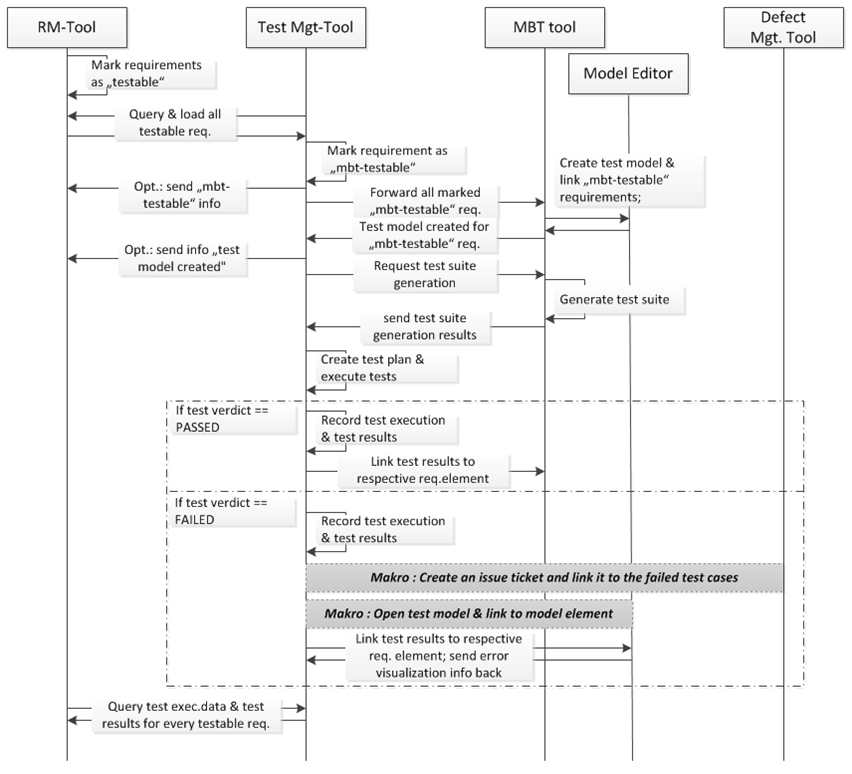
\includegraphics[width=0.65\textwidth]{pics/workflow.png}
	\caption{The to-be-supported workflow using OSLC}
	\label{fig:oslcFW}
\end{figure}


The analysis proceeded with several alternating steps of problem, i.e., environment and need exploration (Step CPS1) and validation of findings by the relevant stakeholders (Steps CPS), until all relevant domains in the problem context and the need were revealed. At this stage of the analysis the problem environment included 27 domains.%, some of the descriptions of which are shown in Figure~\ref{fig:domains}.

%\begin{figure}[htbp]
%	\centering
%	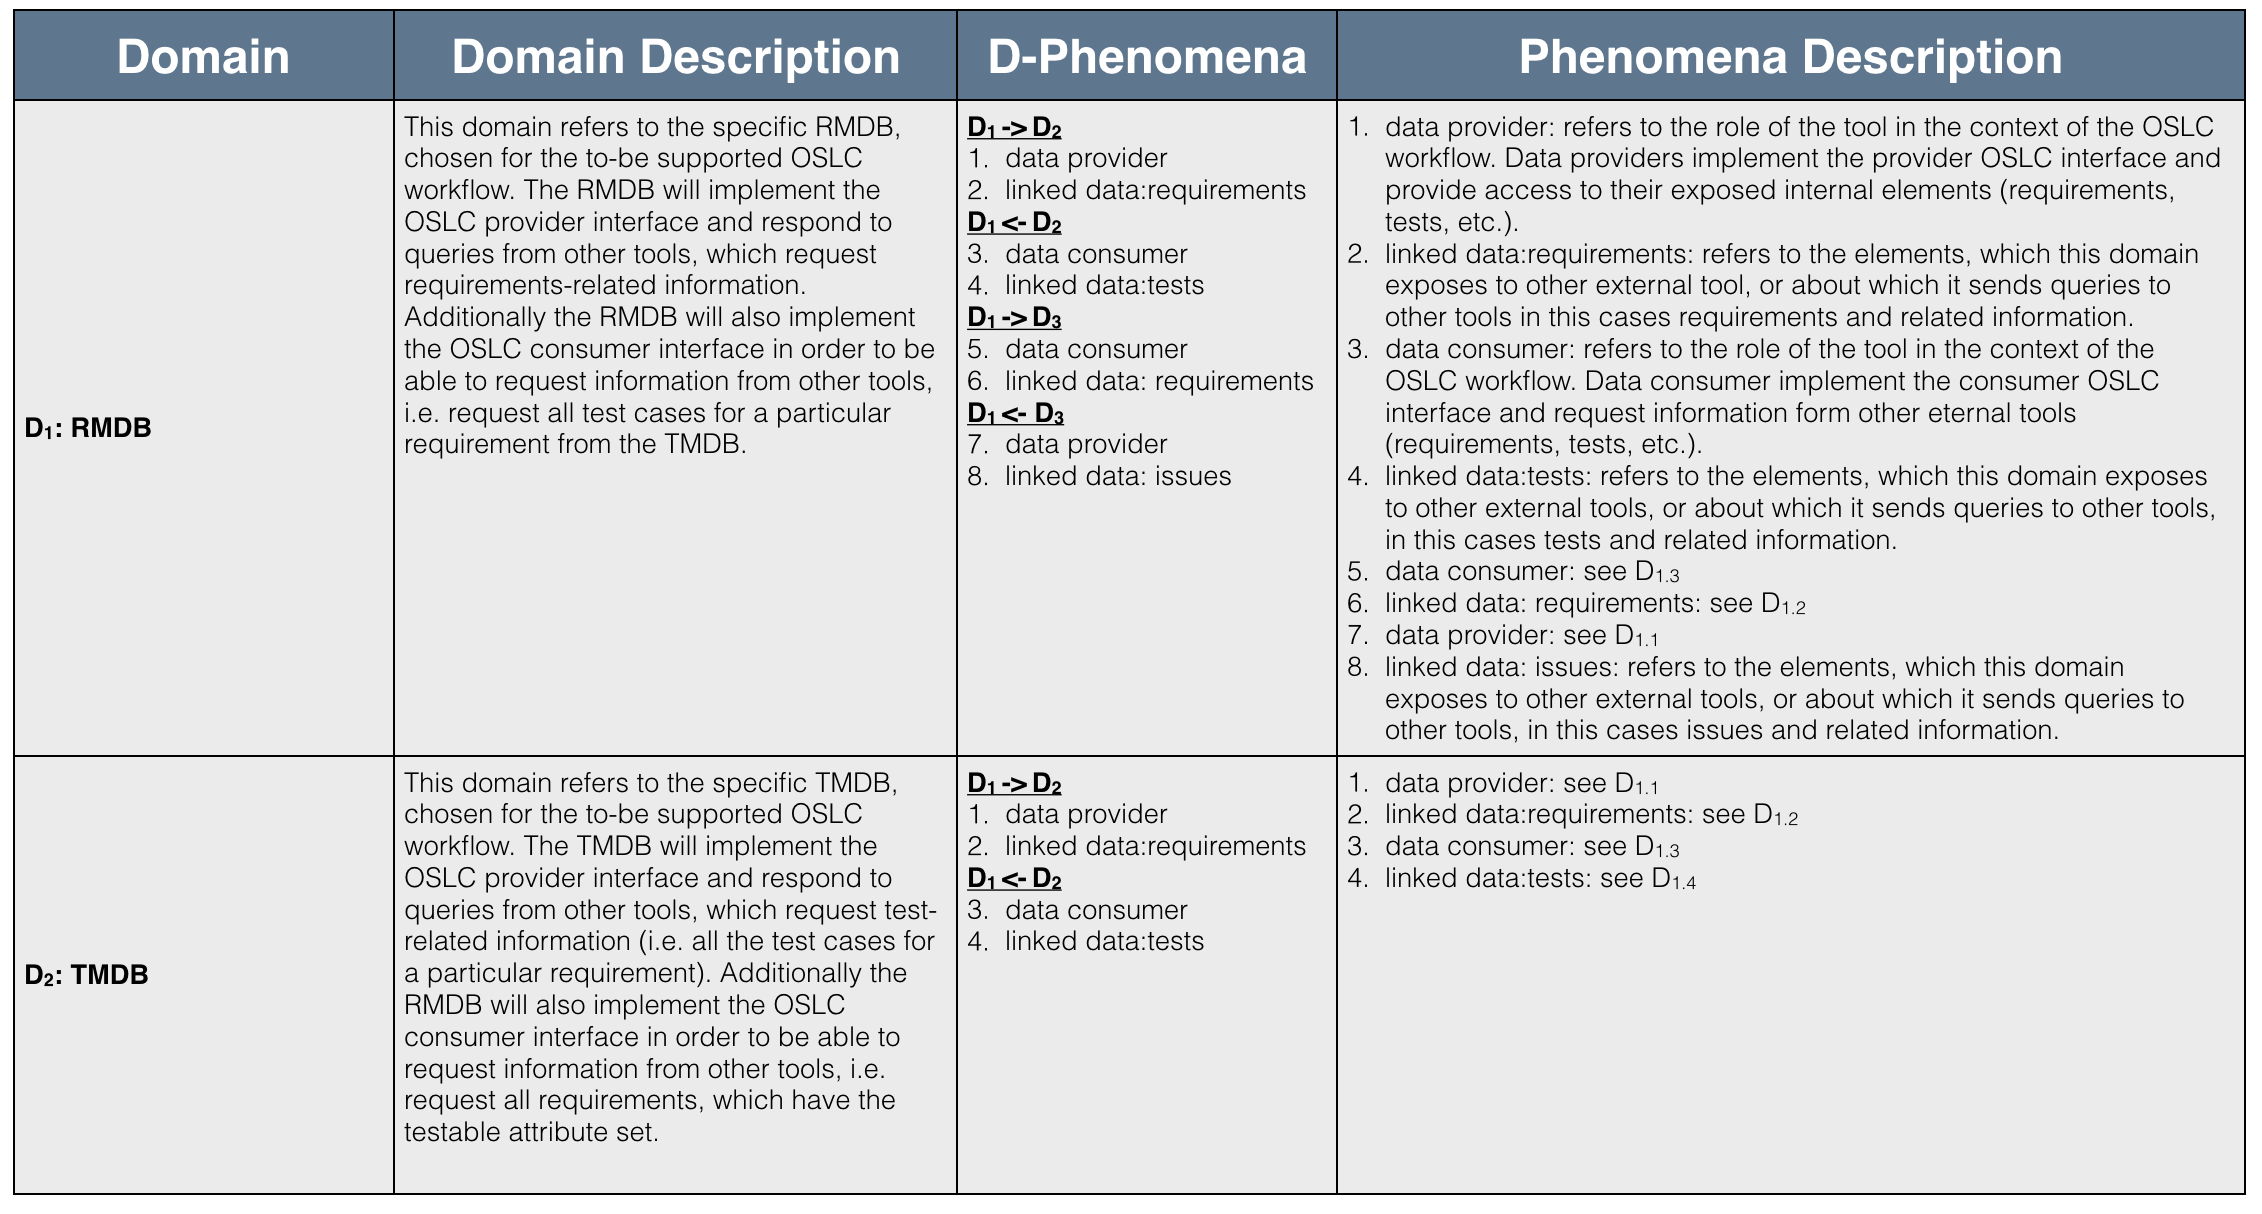
\includegraphics[width=0.75\textwidth]{pics/domains.png}
%	\caption{Domain descriptions}
%	\label{fig:domains}
%\end{figure}

\subsection{Complexity}
This high problem complexity made the change analysis steps (CPS3) very challenging. Due to the many dependencies between exposed environment domains, several of the change artefacts had to be \textit{co-designed}\footnote{\POE{} calls problems that share phenomena in this way tangled problems. Tangled problems are not always susceptible to simple divide and conquer problem solving strategies.}, i.e.,  changes in one domain would have an immediate impact on another domain. Tangled problems are the main reason a classical problem decomposition approach does not always work in complex change problems: such divide and conquer strategy fails to capture the interdependent nature of the sub-problems. An illustrative example of this problem is the latest Apple Watch update. The design of the product required the overcoming the conflicting requirements of adding a new LTE chip inside the watch with the necessary new protocol implementations which require more processing battery power as well as a SIM-card slot, while keeping size and battery life unaffected - a typical HW/SW co-design problem. The next two figures illustrate this problem in the context of our case study. Figure~\ref{fig:tangles} is intended to represent the scale of the problem and to indicated the complex overlaps between domains, expressed through colour codes.

\begin{figure}[htbp]
	\centering
	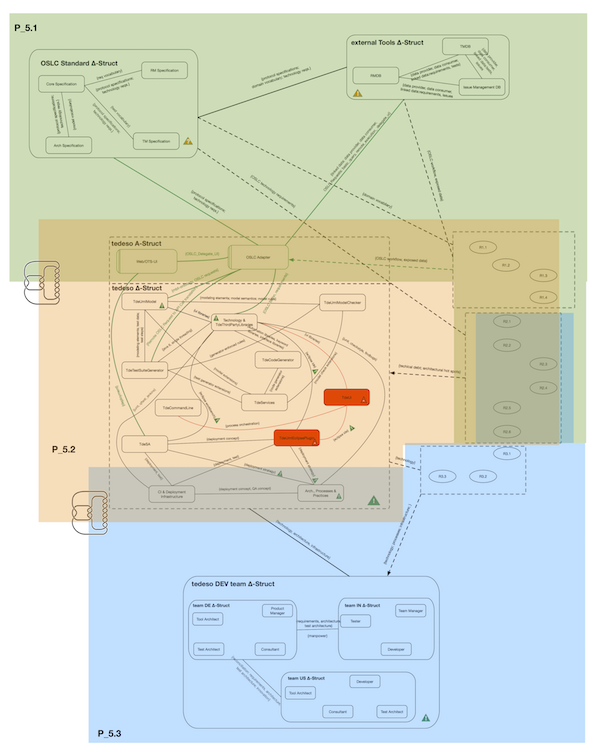
\includegraphics[width=0.47\textwidth]{pics/tangles.png}
	\caption{"The many dependencies between exposed environment domains": green corresponds to external tools/OSLC; blue to the Development organisation; red/orange to the MBT-Tool.}
	\label{fig:tangles}
\end{figure}

Due to the complex tangles, our next step involved isolating the domains on which the tangle depends, design the necessary changes for the remaining domains, and finally reintroducing the changed domains and in a greatly simplified context re-attempt the co-design of the tangled domains. Figure~\ref{fig:pprog} is intended to indicate the complexity of this interaction. An example of such tangle between subproblems is the introduction of several new technologies by one of the distributed teams, i.e. micro-services, etc. as result of the necessary architecture evolution towards supporting the OSLC standard. Since the remaining teams were not familiar with these new technologies, this had an impact on the composition and responsibilities of the other teams as well as introduced the necessity of change (trainings, new hires, etc.) in these domains. 
The co-design of these tangled sub-problems resulted in a successful solution, which during the validation (Step CPS4) was accepted by all stakeholders, including the relevant EU institutions. 

\begin{figure}[htbp]
	\centering
	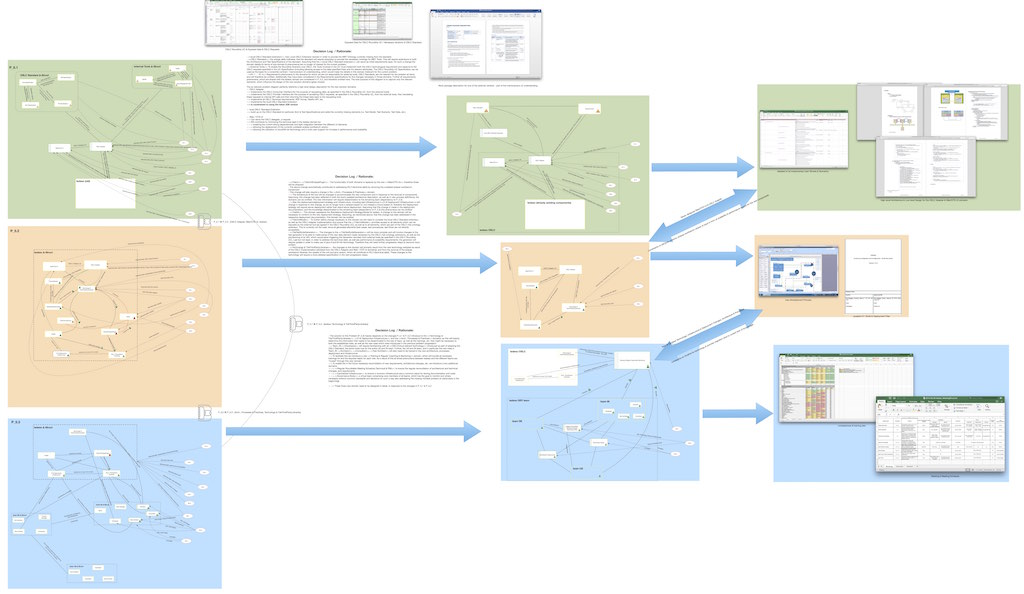
\includegraphics[width=0.95\textwidth]{pics/pprogression.jpg}
	\caption{Handling co-design}
	\label{fig:pprog}
\end{figure}

That is where the study stopped. Step CPS5 --- migrating from original environment $E$ to the newly defined $F$ --- was completed only recently, and long after the case study.

\section{Discussion}\label{sect:Discussion}

The case study work has provided some initial evidence that \POE{}-$\Delta$ is expressive enough for application to a real-world change problem, and able to support the systematisation of its problem solving process. Specifically, in the case study it allowed us to make good progress towards understanding and structuring the initial problem situation, to a point where the problem could be understood by all involved stakeholders, and elements in its context which needed to change could be identified. Further, it provided step-by-step guidance during the change design phase, allowing one to identify clearly: 
%
\begin{enumerate*}[label=(\roman*)]
\item domains that will need to be modified by the solution; 
\item domains that will indirectly influence or be influenced by it or as a result of its introduction to the organisation; and 
\item domains that will remain untouched by the change. 	
\end{enumerate*}

The analysis ended with greenfield problems, to be solved within \POE{}. In fact, the migration between \POE{} and \POE{}-$\Delta$ and back was seamless, thanks to the shared theoretical basis of the two frameworks. It was noted that the framework provides effective tools to focus on specific change subproblems, while still allowing the consideration of co-design issues which are the result of the ways various problem tangle. As such it provides both the means for focussed analysis while reducing the risk of ignoring some important dependences. 

The way the case-study organisation usually handles this type of change problem varies depending on the kind and source of change, but mostly involves some combination of strategic planning, architecture and change management, with high reliance on experts. It was felt by stakeholders that the \POE{}-$\Delta$ approach taken in this case study was able to bring about results comparable to those which might have been obtained through the usual company approach, while increasing the potential for repeatability and reducing reliance on experts. Whether this is actually the case, will be the subject of future studies.

The evaluation also provided some initial findings in regards to the \POE{}-$\Delta$ notation, which was used as a communication medium in most technical meetings. At this technical level, the graphical notation was well understood and its adoption was straightforward. The feedback from the stakeholders was that the use of the graphical notation, instead of its formal counterpart, in the problem analysis steps was crucial to increase the acceptability and learnability of the framework. Additionally, it was felt it helped make structures and relations more explicit and, thus, supported understanding, communication and the discovery of new relationships. In fact, at this technical level the framework was so well received as to be adopted also in other projects. %One participant\footnote{Not a native English speaker} in the project wrote:
%
%\begin{quotation}
%``As I learned and experienced [...] POE-Delta, it helped in systematically approaching one or more changes to an existing [system] where the impact is also for [...] the environment where the solution is to be applied. I have experienced such problems [that POE-Delta addressed] in the past where there are multiple `changes' which also creates some conflicting impact to the existing system. Especially when there are many stakeholders involved. [...] POE-delta can be applied in such cases for a systematic approach for reaching the final goal.

%It could be formally introduced and practiced now.''
%\end{quotation}

The main matter of concern brought up by most stakeholders was the lack of a suitable software tool keep to track of problem models and their relationships, to validate the consistency of problem transformation steps, and provide heuristics or even automation for some intermediate design steps. 

\section{Conclusion}\label{sect:Conclusion}
This paper has introduced POE-$\Delta$, a novel change engineering framework rooted in design and engineering which provides systematic support for representing, structuring and exploring change problems. The paper has discussed its initial formalisation and an early evaluation via a case study concerning technical change in the context of a multi-national organisation, involving many stakeholders. The findings are encouraging, with the framework performing reasonably well in its first full-time application in an industrial setting. 

Current research aims at a full formalisation of the framework on the basis of our work on defining a phenomenal basis for hybrid modelling \cite{hall2017phenomenal}. Additionally, in order to address the main limitation of the case study evaluation reported here - the fact that the POE-$\Delta$ framework was applied by the authors themselves, a more thorough and formal evaluation of the framework is currently in preparation. The evaluation will involve a number of participant from two different countries and at different levels of an organisation. The participant will be separate in two groups - one using the POE-$\Delta$ framework and another, control group, using a state of the art change methodology of their choosing on a common case study. The results of both groups will be compared on a number predefined criteria.

%---------------------------------------------------------------------
%	BIBLIOGRAPHY
%---------------------------------------------------------------------
\frenchspacing
\bibliographystyle{wileyauy}
\bibliography{Literature}

%\begin{thebibliography}{10}
%
%\bibitem{burnes2011success}
%B.~Burnes and P.~Jackson, ``{Success and failure in organizational change: An
%  exploration of the role of values},'' {\em Journal of Change Management},
%  vol.~11, no.~2, pp.~133--162, 2011.
%
%\bibitem{doi:10.1108/14637159910249117}
%G.~Valiris and M.~Glykas, ``Critical review of existing bpr methodologies,''
%  {\em Business Process Management Journal}, vol.~5, no.~1, pp.~65--86, 1999.
%
%\bibitem{Reijers2005283}
%H.~Reijers and S.~L. Mansar, ``Best practices in business process redesign: an
%  overview and qualitative evaluation of successful redesign heuristics,'' {\em
%  Omega}, vol.~33, no.~4, pp.~283 -- 306, 2005.
%
%\bibitem{Gerrits:1994:BMB:646303.686971}
%H.~Gerrits, ``Business modeling based on logistics to support business process
%  re-engineering,'' in {\em Proceedings of the IFIP TC8 Open Conference on
%  Business Process Re-engineering: Information Systems Opportunities and
%  Challenges}, (New York, NY, USA), pp.~279--288, Elsevier Science Inc., 1994.
%
%\bibitem{verkerk2004trust}
%M.~J. Verkerk, {\em {Trust and Power on the Shop Floor: An Ethnographical,
%  Ethical and Philosophical Study on Responsible Behaviour in Industrial
%  Organisations}}.
%\newblock Eburon, 2004.
%
%\bibitem{Kleiner:2000vm}
%A.~Kleiner, ``{Revisiting Reengineering},'' {\em strategy+business}, no.~Third
%  Quarter 2000 / Issue 20, 2000.
%
%\bibitem{By:2005fm}
%R.~T. By, ``{Organisational change management: A critical review},'' {\em
%  Journal of Change Management}, vol.~5, no.~4, pp.~369--380, 2005.
%
%\bibitem{Hall2012ISSE}
%J.~G. Hall and L.~Rapanotti, ``Software engineering as the design theoretic
%  transformation of software problems,'' {\em Innovations in Systems and
%  Software Engineering}, vol.~8, no.~3, pp.~175--193, 2012.
%
%\bibitem{Hevner:2010ua}
%A.~Hevner and S.~Chatterjee, ``{Design Research in Information Systems: Theory
%  and Practice},'' 2010.
%
%\bibitem{Moran:2000ex}
%J.~W. Moran and B.~K. Brightman, ``{Leading organizational change},'' {\em
%  Journal of Workplace Learning}, vol.~12, pp.~66--74, Jan. 2000.
%
%\bibitem{vandeVen:1995uw}
%A.~H. van~de Ven and M.~S. Poole, ``{Explaining development and change in
%  organizations},'' {\em The Academy of Management Review}, vol.~20,
%  pp.~510--540, July 1995.
%
%\bibitem{pettigrew2001studying}
%A.~M. Pettigrew, R.~W. Woodman, and K.~S. Cameron, ``Studying organizational
%  change and development: Challenges for future research,'' {\em Academy of
%  management journal}, vol.~44, no.~4, pp.~697--713, 2001.
%
%\bibitem{Cao:2004dh}
%G.~Cao, S.~Clarke, and B.~Lehaney, ``{The need for a systemic approach to
%  change management{\textemdash}a case study},'' {\em Systemic Practice and
%  Action Research}, 2004.
%
%\bibitem{rowe1991design}
%P.~G. Rowe, {\em Design thinking}.
%\newblock MIT press, 1991.
%
%\bibitem{3460223}
%M.~Eneberg and L.~Svengren~Holm, ``Design thinking and organizational
%  development: twin concepts enabling a reintroduction of democratic values in
%  organizational change,'' EAD - European Academy of Design, 2013.
%
%\bibitem{deserti2014design}
%A.~Deserti and F.~Rizzo, ``Design and organizational change in the public
%  sector,'' {\em Design Management Journal}, vol.~9, no.~1, pp.~85--97, 2014.
%
%\bibitem{jonassen2000toward}
%D.~H. Jonassen, ``Toward a design theory of problem solving,'' {\em Educational
%  technology research and development}, vol.~48, no.~4, pp.~63--85, 2000.
%
%\bibitem{simon1977structure}
%H.~A. Simon, ``The structure of ill-structured problems,'' in {\em Models of
%  discovery}, pp.~304--325, Springer, 1977.
%
%\bibitem{funke1991solving}
%J.~Funke, ``Solving complex problems: Exploration and control of complex
%  systems,'' {\em Complex problem solving: Principles and mechanisms},
%  pp.~185--222, 1991.
%
%\bibitem{smith1993conceptual}
%G.~F. Smith and G.~J. Browne, ``Conceptual foundations of design problem
%  solving,'' {\em Systems, Man and Cybernetics, IEEE Transactions on}, vol.~23,
%  no.~5, pp.~1209--1219, 1993.
%
%\bibitem{martin2009design}
%R.~L. Martin, {\em The design of business: why design thinking is the next
%  competitive advantage}.
%\newblock Harvard Business Press, 2009.
%
%\bibitem{leavy2010design}
%B.~Leavy, ``Design thinking--a new mental model of value innovation,'' {\em
%  Strategy \& leadership}, vol.~38, no.~3, pp.~5--14, 2010.
%
%\bibitem{Hall2009JAdvSysMeas}
%J.~G. Hall and L.~Rapanotti, ``Assurance-driven design in problem oriented
%  engineering,'' {\em International Journal on Advances in Systems and
%  Measurements}, vol.~2, October, 26-31 2009.
%\newblock http://oro.open.ac.uk/19123/.
%
%\bibitem{hall2016a-design}
%J.~G. Hall and L.~Rapanotti, ``A design theory for software engineering,''
%  Technical Report TR2016/01, Department of Computing and Communications, The
%  Open University, Walton Hall, Milton Keynes, MK7 6AA, 2016.
%
%\bibitem{896248}
%C.~Gunter, E.~Gunter, M.~Jackson, and P.~Zave, ``A reference model for
%  requirements and specifications,'' {\em Software, IEEE}, vol.~17, pp.~37--43,
%  May 2000.
%
%\bibitem{Jackson2001}
%M.~A. Jackson, {\em Problem Frames: Analyzing and Structuring Software
%  Development Problem}.
%\newblock Addison-Wesley Publishing Company, 1st~ed., 2001.
%
%\bibitem{hall2003reference}
%J.~G. Hall and L.~Rapanotti, ``A reference model for requirements
%  engineering,'' in {\em Requirements Engineering Conference, 2003.
%  Proceedings. 11th IEEE International}, pp.~181--187, IEEE, 2003.
%
%\bibitem{weick1995sensemaking}
%K.~E. Weick, {\em Sensemaking in organizations}, vol.~3.
%\newblock Sage, 1995.
%
%\bibitem{rogers1983nature}
%G.~Rogers, {\em The nature of engineering: a philosophy of technology}.
%\newblock Macmillan Press, 1983.
%
%\bibitem{1999:RID:311424}
%{\em Refactoring: Improving the Design of Existing Code}.
%\newblock Boston, MA, USA: Addison-Wesley Longman Publishing Co., Inc., 1999.
%
%\end{thebibliography}
\end{document}
